% !TEX program = pdflatex
\documentclass[aspectratio=169,11pt]{beamer}

% ─── Theme & Colors ───────────────────────────────────────────────────
\usetheme{Madrid}
\usecolortheme{default}

\definecolor{primary}{HTML}{2563EB}
\definecolor{secondary}{HTML}{7C3AED}
\definecolor{accent}{HTML}{059669}
\definecolor{warning}{HTML}{D97706}
\definecolor{danger}{HTML}{DC2626}
\definecolor{darkbg}{HTML}{1E293B}
\definecolor{lightbg}{HTML}{F1F5F9}
\definecolor{gentlegray}{HTML}{64748B}

\setbeamercolor{palette primary}{bg=primary,fg=white}
\setbeamercolor{palette secondary}{bg=secondary,fg=white}
\setbeamercolor{palette tertiary}{bg=darkbg,fg=white}
\setbeamercolor{structure}{fg=primary}
\setbeamercolor{title}{fg=white,bg=primary}
\setbeamercolor{frametitle}{fg=white,bg=primary}
\setbeamercolor{block title}{bg=primary!15,fg=primary!80!black}
\setbeamercolor{block body}{bg=primary!5}
\setbeamercolor{block title alerted}{bg=danger!15,fg=danger!80!black}
\setbeamercolor{block body alerted}{bg=danger!5}
\setbeamercolor{block title example}{bg=accent!15,fg=accent!80!black}
\setbeamercolor{block body example}{bg=accent!5}
\setbeamercolor{itemize item}{fg=primary}
\setbeamercolor{itemize subitem}{fg=secondary}
\setbeamercolor{enumerate item}{fg=primary}

\setbeamertemplate{navigation symbols}{}
\setbeamertemplate{footline}[frame number]

% ─── Packages ─────────────────────────────────────────────────────────
\usepackage{tikz}
\usetikzlibrary{
  shapes.geometric, arrows.meta, positioning, calc,
  fit, backgrounds, decorations.pathreplacing
}
\usepackage[utf8]{inputenc}
\usepackage[T1]{fontenc}
\usepackage{booktabs}
\usepackage{graphicx}
\usepackage{hyperref}
\usepackage{amsmath}

% ─── TikZ Styles ─────────────────────────────────────────────────────
\tikzset{
  box/.style={
    draw=#1!60, fill=#1!8, rounded corners=4pt,
    minimum height=0.85cm, font=\scriptsize\sffamily,
    text=darkbg, align=center
  },
  box/.default=primary,
  wbox/.style={
    draw=#1!60, fill=#1!8, rounded corners=6pt,
    minimum height=1cm, font=\small\sffamily,
    text=darkbg, align=center, inner sep=8pt
  },
  wbox/.default=primary,
  arr/.style={-{Stealth[length=5pt,width=4pt]}, thick, color=#1!60},
  arr/.default=primary,
  darr/.style={-{Stealth[length=5pt,width=4pt]}, dashed, thick, color=#1!45},
  darr/.default=gentlegray,
  lbl/.style={font=\tiny\sffamily, text=gentlegray},
}

% ─── Title ────────────────────────────────────────────────────────────
\title[TeacherLM]{\textbf{TeacherLM}}
\subtitle{Pr\'esentation d'\'{E}tat d'Avancement\\[4pt]
{\small Syst\`eme Multi-Agents RAG pour le Tutorat Intelligent}}
\author{}
\date{\today}
\institute{}

% ══════════════════════════════════════════════════════════════════════
\begin{document}

% ─── TITRE ────────────────────────────────────────────────────────────
{
\setbeamertemplate{footline}{}
\begin{frame}
\titlepage
\end{frame}
}

% ─── PLAN ─────────────────────────────────────────────────────────────
\begin{frame}{Plan}
\tableofcontents
\end{frame}

% ══════════════════════════════════════════════════════════════════════
\section{Contexte et Probl\'ematique}
% ══════════════════════════════════════════════════════════════════════

\begin{frame}{Contexte et Probl\'ematique}
\begin{columns}[T]
\begin{column}{0.48\textwidth}
  \begin{block}{Le probl\`eme}
    Les LLM (\textbf{Large Language Models}) sont puissants, mais~:
    \begin{itemize}
      \item Ils \textbf{hallucinent} --- ils inventent des informations
      \item Ils ne connaissent pas \textbf{vos} supports de cours
      \item Ils ne s'adaptent pas au \textbf{niveau de l'\'{e}tudiant}
    \end{itemize}
  \end{block}

  \bigskip
  \begin{alertblock}{Objectif de TeacherLM}
    Construire un tuteur IA qui r\'epond \textbf{uniquement} \`a partir des documents fournis par l'\'{e}tudiant, en s'adaptant \`a son niveau.
  \end{alertblock}
\end{column}
\begin{column}{0.48\textwidth}
  \begin{block}{Notre approche}
    Combiner trois techniques~:
    \begin{enumerate}
      \item \textbf{RAG} --- ancrer les r\'eponses dans les documents
      \item \textbf{Multi-agents} --- des agents sp\'ecialis\'es pour chaque t\^ache
      \item \textbf{Suivi apprenant} --- mod\`ele de ma\^itrise par concept
    \end{enumerate}
  \end{block}

  \bigskip
  \begin{exampleblock}{R\'esultat}
    L'\'{e}tudiant t\'el\'everse ses PDF, puis~:
    \begin{itemize}
      \item \textbf{Chat} avec un enseignant IA
      \item \textbf{Quiz} adaptatifs
      \item \textbf{Flashcards} avec r\'ep\'etition espac\'ee
    \end{itemize}
  \end{exampleblock}
\end{column}
\end{columns}
\end{frame}

% ══════════════════════════════════════════════════════════════════════
\section{Qu'est-ce que le RAG~?}
% ══════════════════════════════════════════════════════════════════════

\begin{frame}{Qu'est-ce que le RAG~?}
\textbf{RAG} = \textbf{R}etrieval-\textbf{A}ugmented \textbf{G}eneration (G\'en\'eration Augment\'ee par R\'ecup\'eration).

\bigskip
\begin{columns}[T]
\begin{column}{0.55\textwidth}
  \begin{block}{Principe}
    Au lieu de demander directement au LLM de r\'epondre~:
    \begin{enumerate}
      \item On \textbf{cherche} les passages pertinents dans les documents
      \item On les \textbf{injecte} dans le prompt du LLM
      \item Le LLM r\'epond en se basant \textbf{uniquement} sur ces passages
    \end{enumerate}
  \end{block}

  \bigskip
  \begin{exampleblock}{Pourquoi le RAG~?}
    \begin{itemize}
      \item \'Elimine les \textbf{hallucinations} --- le LLM ne peut r\'epondre que depuis les documents
      \item Pas besoin de \textbf{r\'e-entra\^iner} le mod\`ele
      \item Les r\'eponses sont \textbf{tra\c{c}ables} (on sait d'o\`u vient chaque fait)
    \end{itemize}
  \end{exampleblock}
\end{column}
\begin{column}{0.42\textwidth}
  \centering
  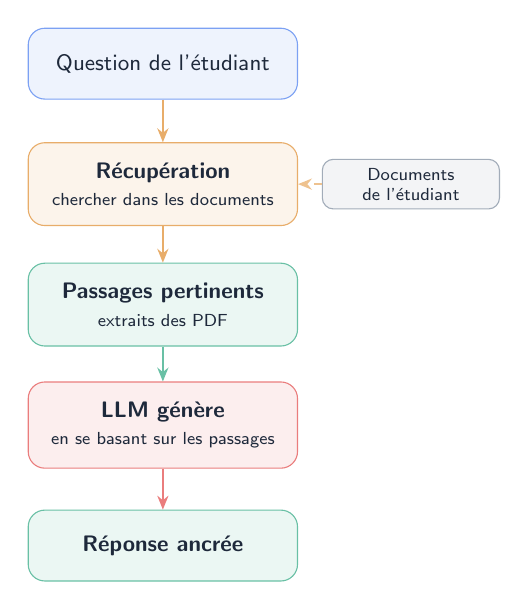
\begin{tikzpicture}[scale=0.9, every node/.style={transform shape}]
    \node[wbox=primary, minimum width=3.8cm] (q) at (0,4.5) {Question de l'\'{e}tudiant};

    \node[wbox=warning, minimum width=3.8cm] (ret) at (0,2.8)
      {\textbf{R\'ecup\'eration}\\{\scriptsize chercher dans les documents}};

    \node[wbox=accent, minimum width=3.8cm] (ctx) at (0,1.1)
      {\textbf{Passages pertinents}\\{\scriptsize extraits des PDF}};

    \node[wbox=danger, minimum width=3.8cm] (llm) at (0,-0.6)
      {\textbf{LLM g\'en\`ere}\\{\scriptsize en se basant sur les passages}};

    \node[wbox=accent, minimum width=3.8cm] (ans) at (0,-2.3)
      {\textbf{R\'eponse ancr\'ee}};

    \draw[arr=warning] (q) -- (ret);
    \draw[arr=warning] (ret) -- (ctx);
    \draw[arr=accent] (ctx) -- (llm);
    \draw[arr=danger] (llm) -- (ans);

    \node[box=gentlegray, minimum width=2.5cm, minimum height=0.7cm]
      (docs) at (3.5,2.8) {Documents\\de l'\'{e}tudiant};
    \draw[darr=warning] (docs) -- (ret);
  \end{tikzpicture}
\end{column}
\end{columns}
\end{frame}

% ══════════════════════════════════════════════════════════════════════
\section{Architecture G\'en\'erale}
% ══════════════════════════════════════════════════════════════════════

\begin{frame}{Architecture G\'en\'erale du Syst\`eme}
\centering
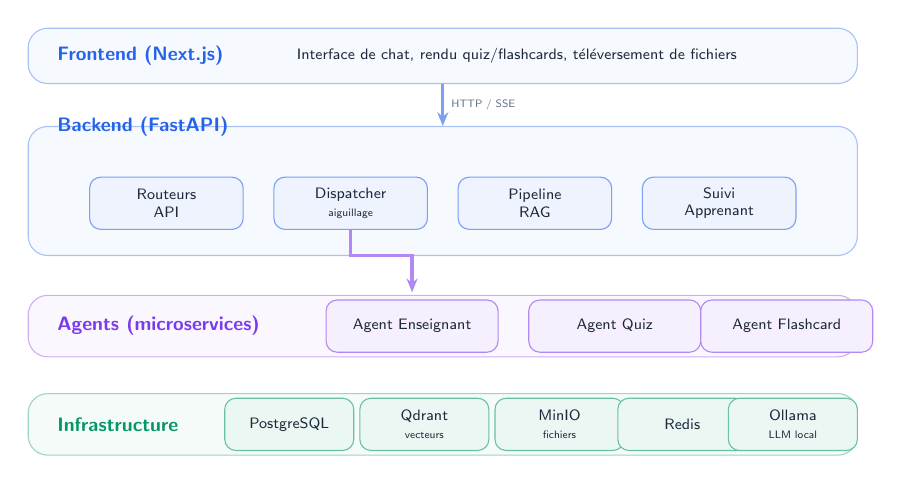
\begin{tikzpicture}[scale=0.78, every node/.style={transform shape}]
  % Frontend
  \node[draw=primary!40, fill=primary!4, rounded corners=7pt,
        minimum width=13.5cm, minimum height=0.9cm]
    (fe) at (0,5.2) {};
  \node[font=\small\sffamily\bfseries, text=primary, anchor=west]
    at (-6.4,5.2) {Frontend (Next.js)};
  \node[font=\scriptsize\sffamily, text=darkbg, anchor=west]
    at (-2.5,5.2) {Interface de chat, rendu quiz/flashcards, t\'el\'eversement de fichiers};

  % Backend
  \node[draw=primary!40, fill=primary!4, rounded corners=7pt,
        minimum width=13.5cm, minimum height=2.1cm]
    (be) at (0,3) {};
  \node[font=\small\sffamily\bfseries, text=primary, anchor=west]
    at (-6.4,4.05) {Backend (FastAPI)};

  \node[box=primary, minimum width=2.5cm] at (-4.5,2.8) {Routeurs\\API};
  \node[box=primary, minimum width=2.5cm] (disp) at (-1.5,2.8) {Dispatcher\\{\tiny aiguillage}};
  \node[box=primary, minimum width=2.5cm] at (1.5,2.8) {Pipeline\\RAG};
  \node[box=primary, minimum width=2.5cm] at (4.5,2.8) {Suivi\\Apprenant};

  % Agents
  \node[draw=secondary!40, fill=secondary!4, rounded corners=7pt,
        minimum width=13.5cm, minimum height=1cm]
    (ag) at (0,0.8) {};
  \node[font=\small\sffamily\bfseries, text=secondary, anchor=west]
    at (-6.4,0.8) {Agents (microservices)};
  \node[box=secondary, minimum width=2.8cm] at (-0.5,0.8) {Agent Enseignant};
  \node[box=secondary, minimum width=2.8cm] at (2.8,0.8) {Agent Quiz};
  \node[box=secondary, minimum width=2.8cm] at (5.6,0.8) {Agent Flashcard};

  % Infra
  \node[draw=accent!40, fill=accent!4, rounded corners=7pt,
        minimum width=13.5cm, minimum height=1cm]
    (inf) at (0,-0.8) {};
  \node[font=\small\sffamily\bfseries, text=accent, anchor=west]
    at (-6.4,-0.8) {Infrastructure};
  \node[box=accent, minimum width=2.1cm] at (-2.5,-0.8) {PostgreSQL};
  \node[box=accent, minimum width=2.1cm] at (-0.3,-0.8) {Qdrant\\{\tiny vecteurs}};
  \node[box=accent, minimum width=2.1cm] at (1.9,-0.8) {MinIO\\{\tiny fichiers}};
  \node[box=accent, minimum width=2.1cm] at (3.9,-0.8) {Redis};
  \node[box=accent, minimum width=2.1cm] at (5.7,-0.8) {Ollama\\{\tiny LLM local}};

  % Arrows
  \draw[arr, line width=1.2pt] (fe) -- node[right, lbl] {HTTP / SSE} (be);
  \draw[arr=secondary, line width=1.2pt] (disp) -- ++(0,-0.85) -| (-0.5,1.35);
\end{tikzpicture}

\bigskip
\begin{columns}[T]
\begin{column}{0.46\textwidth}
  \begin{block}{Composant cl\'e~: Ollama}
    Ollama ex\'ecute les mod\`eles LLM \textbf{localement} sur la machine.
    Aucune donn\'ee ne part vers le cloud $\rightarrow$ \textbf{confidentialit\'e totale}.
  \end{block}
\end{column}
\begin{column}{0.46\textwidth}
  \begin{block}{Composant cl\'e~: Qdrant}
    Base de donn\'ees \textbf{vectorielle} --- stocke les repr\'esentations num\'eriques des passages de texte pour la recherche s\'emantique.
  \end{block}
\end{column}
\end{columns}
\end{frame}

% ══════════════════════════════════════════════════════════════════════
\section{Pipeline RAG --- Ingestion}
% ══════════════════════════════════════════════════════════════════════

\begin{frame}{Pipeline RAG --- Phase d'Ingestion}

Quand l'\'{e}tudiant t\'el\'everse un fichier PDF, le syst\`eme le pr\'epare en 4 \'etapes~:

\bigskip
\centering
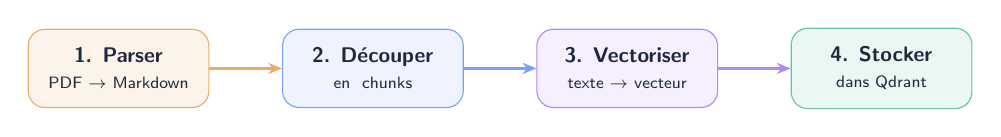
\begin{tikzpicture}[scale=0.85, every node/.style={transform shape}]
  \node[wbox=warning, minimum width=2.7cm] (s1) at (0,0)
    {\textbf{1. Parser}\\{\scriptsize PDF $\rightarrow$ Markdown}};
  \node[wbox=primary, minimum width=2.7cm] (s2) at (3.8,0)
    {\textbf{2. D\'ecouper}\\{\scriptsize en \og{} chunks \fg{}}};
  \node[wbox=secondary, minimum width=2.7cm] (s3) at (7.6,0)
    {\textbf{3. Vectoriser}\\{\scriptsize texte $\rightarrow$ vecteur}};
  \node[wbox=accent, minimum width=2.7cm] (s4) at (11.4,0)
    {\textbf{4. Stocker}\\{\scriptsize dans Qdrant}};

  \draw[arr=warning, line width=1.2pt] (s1) -- (s2);
  \draw[arr=primary, line width=1.2pt] (s2) -- (s3);
  \draw[arr=secondary, line width=1.2pt] (s3) -- (s4);
\end{tikzpicture}

\bigskip
\begin{columns}[T]
\begin{column}{0.46\textwidth}
  \begin{block}{\'Etape 1~: Parsing (LlamaCloud)}
    Les PDF contiennent des tableaux, colonnes, \'equations. \textbf{LlamaCloud} les convertit en \textbf{Markdown propre} --- un format texte structur\'e, facile \`a d\'ecouper.
  \end{block}

  \begin{block}{\'Etape 2~: Chunking (d\'ecoupage)}
    Le Markdown est d\'ecoup\'e en \textbf{chunks} (morceaux) de $\sim$512 tokens.

    \smallskip
    {\small\textbf{Pourquoi~?} Les LLM ont une fen\^etre de contexte limit\'ee. On ne peut pas injecter un document entier --- on injecte les \emph{morceaux pertinents}.}

    \smallskip
    {\small \textbf{Chevauchement de 50 tokens}  entre chunks cons\'ecutifs pour ne pas couper une id\'ee en deux.}
  \end{block}
\end{column}
\begin{column}{0.46\textwidth}
  \begin{block}{\'Etape 3~: Embedding (vectorisation)}
    Chaque chunk est transform\'e en un \textbf{vecteur} (liste de 384 nombres) par le mod\`ele \texttt{BGE-small}.

    \smallskip
    {\small \textbf{Qu'est-ce qu'un embedding~?} C'est une repr\'esentation num\'erique du \emph{sens} d'un texte. Deux textes s\'emantiquement proches auront des vecteurs proches dans l'espace vectoriel.}
  \end{block}

  \begin{block}{\'Etape 4~: Stockage (Qdrant)}
    Les vecteurs sont stock\'es dans \textbf{Qdrant}, une base de donn\'ees vectorielle.

    \smallskip
    {\small Chaque conversation a sa \textbf{propre collection} --- isolation compl\`ete entre les \'etudiants.}
  \end{block}
\end{column}
\end{columns}
\end{frame}

% ══════════════════════════════════════════════════════════════════════
\section{Pipeline RAG --- R\'ecup\'eration}
% ══════════════════════════════════════════════════════════════════════

\begin{frame}{Pipeline RAG --- Phase de R\'ecup\'eration}

Quand l'\'{e}tudiant pose une question, le syst\`eme recherche les passages les plus pertinents~:

\bigskip
\centering
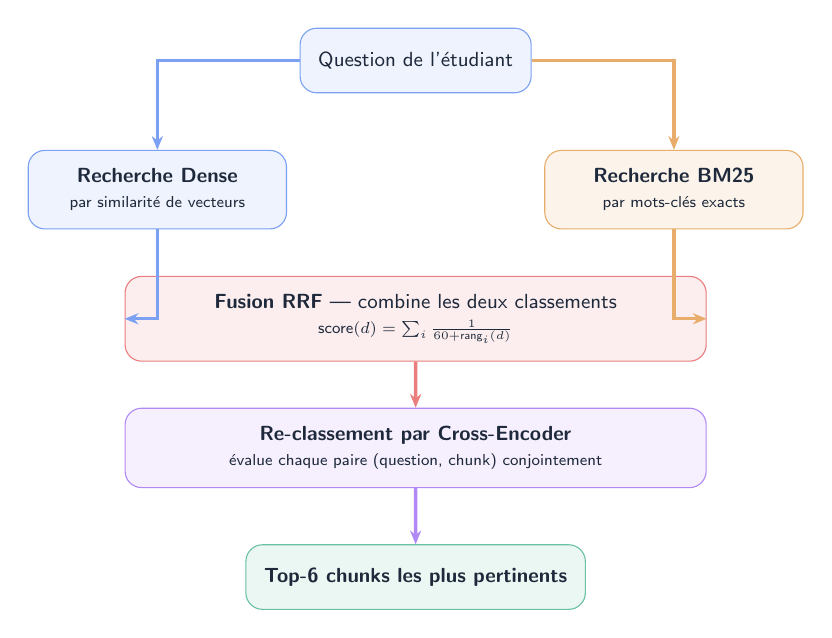
\begin{tikzpicture}[scale=0.82, every node/.style={transform shape}]
  % Query
  \node[wbox=primary, minimum width=3.5cm] (q) at (0,3) {Question de l'\'{e}tudiant};

  % Branches
  \node[wbox=primary, minimum width=4cm] (dense) at (-4,1)
    {\textbf{Recherche Dense}\\{\scriptsize par similarit\'e de vecteurs}};
  \node[wbox=warning, minimum width=4cm] (sparse) at (4,1)
    {\textbf{Recherche BM25}\\{\scriptsize par mots-cl\'es exacts}};

  % RRF
  \node[wbox=danger, minimum width=9cm] (rrf) at (0,-1)
    {\textbf{Fusion RRF} --- combine les deux classements\\
     {\scriptsize $\text{score}(d) = \sum_i \frac{1}{60 + \text{rang}_i(d)}$}};

  % Reranker
  \node[wbox=secondary, minimum width=9cm] (rr) at (0,-3)
    {\textbf{Re-classement par Cross-Encoder}\\
     {\scriptsize \'evalue chaque paire (question, chunk) conjointement}};

  % Output
  \node[wbox=accent, minimum width=4cm] (out) at (0,-5)
    {\textbf{Top-6 chunks les plus pertinents}};

  \draw[arr, line width=1.2pt] (q) -| (dense);
  \draw[arr=warning, line width=1.2pt] (q) -| (sparse);
  \draw[arr, line width=1.2pt] (dense) |- (rrf);
  \draw[arr=warning, line width=1.2pt] (sparse) |- (rrf);
  \draw[arr=danger, line width=1.2pt] (rrf) -- (rr);
  \draw[arr=secondary, line width=1.2pt] (rr) -- (out);
\end{tikzpicture}
\end{frame}

% ──────────────────────────────────────────────────────────────────────
\begin{frame}{Explication des Techniques de R\'ecup\'eration}
\begin{columns}[T]
\begin{column}{0.48\textwidth}
  \begin{block}{Recherche Dense (s\'emantique)}
    On transforme la question en vecteur (embedding), puis on cherche les vecteurs les plus \textbf{proches} dans Qdrant.

    \smallskip
    {\small \textbf{Force~:} comprend le \emph{sens}. ``Qu'est-ce qui cause la rouille~?'' trouve ``l'oxydation du fer''.}

    \smallskip
    {\small \textbf{Faiblesse~:} peut rater des termes exacts sp\'ecialis\'es.}
  \end{block}

  \bigskip
  \begin{block}{Recherche BM25 (mots-cl\'es)}
    \textbf{BM25} est un algorithme classique de recherche par mots-cl\'es (utilis\'e par les moteurs de recherche).

    \smallskip
    {\small \textbf{Force~:} trouve les correspondances \emph{exactes}. ``\'equation de Henderson-Hasselbalch'' $\rightarrow$ match direct.}

    \smallskip
    {\small \textbf{Faiblesse~:} ne comprend pas les synonymes.}
  \end{block}
\end{column}
\begin{column}{0.48\textwidth}
  \begin{block}{Fusion RRF (Reciprocal Rank Fusion)}
    On combine les r\'esultats des deux recherches. Chaque document re\c{c}oit un score bas\'e sur son \textbf{rang} dans chaque liste.

    \smallskip
    {\small \textbf{Pourquoi~?} La recherche dense et BM25 se compl\`etent. RRF capte \`a la fois le sens \emph{et} les mots-cl\'es.}
  \end{block}

  \bigskip
  \begin{block}{Cross-Encoder (re-classement)}
    Un mod\`ele sp\'ecialis\'e (\texttt{bge-reranker-base}) qui \'evalue chaque paire \textbf{(question, chunk)} conjointement.

    \smallskip
    {\small \textbf{Diff\'erence avec l'embedding~:} l'embedding encode question et chunk \emph{s\'epar\'ement}. Le cross-encoder les lit \emph{ensemble} $\rightarrow$ beaucoup plus pr\'ecis, mais aussi plus lent.}

    \smallskip
    {\small On l'utilise sur les $\sim$20 meilleurs candidats pour s\'electionner les \textbf{top 6}.}
  \end{block}
\end{column}
\end{columns}
\end{frame}

% ──────────────────────────────────────────────────────────────────────
\begin{frame}{Technique Avanc\'ee~: HyDE}
\begin{columns}[T]
\begin{column}{0.52\textwidth}
  \textbf{HyDE} = \textbf{Hy}pothetical \textbf{D}ocument \textbf{E}mbeddings.

  \bigskip
  \begin{block}{Le probl\`eme r\'esolu}
    Les \'etudiants posent des questions en langage \textbf{familier}.
    Les documents utilisent un langage \textbf{acad\'emique}.

    \smallskip
    \emph{``Pourquoi les trucs rouillent~?''} vs. \emph{``L'oxydation du fer se produit en pr\'esence d'eau et d'oxyg\`ene\ldots''}
    
    \smallskip
    La similarit\'e vectorielle entre ces deux textes peut \^etre faible.
  \end{block}

  \bigskip
  \begin{block}{La solution HyDE}
    \begin{enumerate}
      \item Le LLM g\'en\`ere une \textbf{r\'eponse hypoth\'etique} \`a la question (en langage acad\'emique)
      \item On utilise cette r\'eponse pour am\'eliorer la recherche
      \item Le cross-encoder compare les chunks \`a \textbf{question + hypoth\`ese}
    \end{enumerate}

    \smallskip
    {\small R\'esultat~: on \textbf{comble l'\'ecart de vocabulaire} entre l'\'etudiant et le cours.}
  \end{block}
\end{column}
\begin{column}{0.44\textwidth}
  \centering
  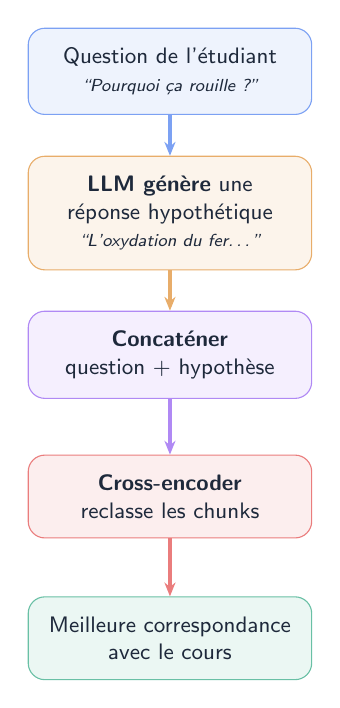
\begin{tikzpicture}[scale=0.9, every node/.style={transform shape}]
    \node[wbox=primary, minimum width=4cm] (q) at (0,5)
      {Question de l'\'etudiant\\{\scriptsize\emph{``Pourquoi \c{c}a rouille~?''}}};

    \node[wbox=warning, minimum width=4cm] (hyde) at (0,3)
      {\textbf{LLM g\'en\`ere} une\\r\'eponse hypoth\'etique\\
       {\scriptsize\emph{``L'oxydation du fer\ldots''}}};

    \node[wbox=secondary, minimum width=4cm] (cat) at (0,1)
      {\textbf{Concat\'ener}\\question + hypoth\`ese};

    \node[wbox=danger, minimum width=4cm] (ce) at (0,-1)
      {\textbf{Cross-encoder}\\reclasse les chunks};

    \node[wbox=accent, minimum width=4cm] (out) at (0,-3)
      {Meilleure correspondance\\avec le cours};

    \draw[arr=primary, line width=1.2pt] (q) -- (hyde);
    \draw[arr=warning, line width=1.2pt] (hyde) -- (cat);
    \draw[arr=secondary, line width=1.2pt] (cat) -- (ce);
    \draw[arr=danger, line width=1.2pt] (ce) -- (out);
  \end{tikzpicture}
\end{column}
\end{columns}
\end{frame}

% ══════════════════════════════════════════════════════════════════════
\section{Les Agents}
% ══════════════════════════════════════════════════════════════════════

\begin{frame}{Qu'est-ce qu'un Agent dans TeacherLM~?}
\begin{columns}[T]
\begin{column}{0.48\textwidth}
  \begin{block}{D\'efinition}
    Un \textbf{agent} est un microservice autonome qui~:
    \begin{itemize}
      \item Re\c{c}oit les chunks du pipeline RAG
      \item Re\c{c}oit l'\'{e}tat de l'apprenant
      \item Ex\'ecute un \textbf{pipeline multi-\'etapes} propre \`a sa t\^ache
      \item Produit un r\'esultat sp\'ecialis\'e
    \end{itemize}
  \end{block}

  \bigskip
  \begin{block}{Architecture Plugin}
    Chaque agent est un \textbf{service ind\'ependant} avec~:
    \begin{itemize}
      \item Son propre conteneur Docker
      \item Ses propres prompts
      \item Sa propre configuration de mod\`eles
    \end{itemize}

    \smallskip
    {\small \textbf{Ajout d'un agent~:} cr\'eer un nouveau service + l'enregistrer dans un fichier JSON. Z\'ero modification du backend.}
  \end{block}
\end{column}
\begin{column}{0.48\textwidth}
  \centering
  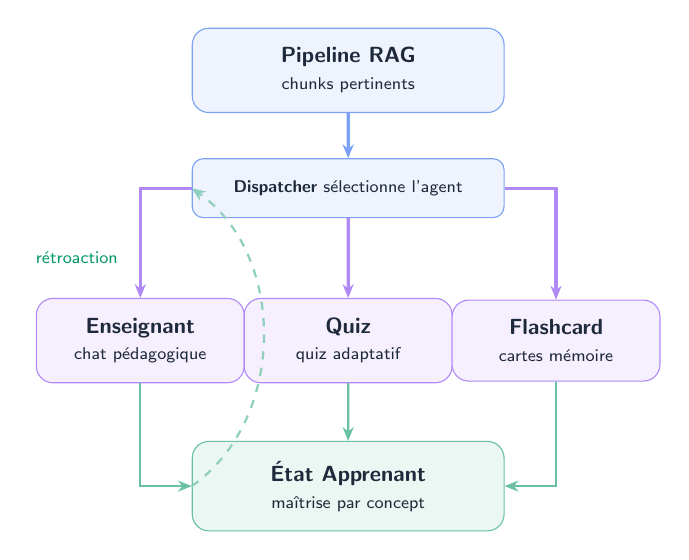
\begin{tikzpicture}[scale=0.88, every node/.style={transform shape}]
    \node[wbox=primary, minimum width=4.5cm] (rag) at (0,4.5)
      {\textbf{Pipeline RAG}\\{\scriptsize chunks pertinents}};

    \node[box=primary, minimum width=4.5cm, minimum height=0.85cm] (disp) at (0,2.8)
      {\textbf{Dispatcher} s\'electionne l'agent};

    \node[wbox=secondary, minimum width=3cm] (t) at (-3,0.6)
      {\textbf{Enseignant}\\{\scriptsize chat p\'edagogique}};
    \node[wbox=secondary, minimum width=3cm] (q) at (0,0.6)
      {\textbf{Quiz}\\{\scriptsize quiz adaptatif}};
    \node[wbox=secondary, minimum width=3cm] (f) at (3,0.6)
      {\textbf{Flashcard}\\{\scriptsize cartes m\'emoire}};

    \node[wbox=accent, minimum width=4.5cm] (ls) at (0,-1.5)
      {\textbf{\'Etat Apprenant}\\{\scriptsize ma\^itrise par concept}};

    \draw[arr, line width=1.2pt] (rag) -- (disp);
    \draw[arr=secondary, line width=1.2pt] (disp) -| (t);
    \draw[arr=secondary, line width=1.2pt] (disp) -- (q);
    \draw[arr=secondary, line width=1.2pt] (disp) -| (f);
    \draw[arr=accent] (t) |- (ls);
    \draw[arr=accent] (q) -- (ls);
    \draw[arr=accent] (f) |- (ls);
    \draw[darr=accent, bend right=55] (ls.west) to (disp.west);
    \node[lbl, text=accent, anchor=east] at (-3.2,1.8) {\scriptsize r\'etroaction};
  \end{tikzpicture}
\end{column}
\end{columns}
\end{frame}

% ══════════════════════════════════════════════════════════════════════
\subsection{Agent Enseignant}
% ══════════════════════════════════════════════════════════════════════

\begin{frame}{Agent Enseignant --- Le C\oe{}ur du Syst\`eme}
\begin{columns}[T]
\begin{column}{0.48\textwidth}
  C'est l'agent principal~: il r\'epond aux questions de l'\'etudiant comme un \textbf{enseignant bienveillant et patient}.

  \bigskip
  \begin{block}{Pipeline en 6 \'etapes}
    \begin{enumerate}
      \item \textbf{Analyser la question} --- le LLM (3B, rapide) extrait~: l'intention, le niveau de confusion (0--1), le concept cible.

      \item \textbf{Choisir le mode} --- un arbre de d\'ecision s\'electionne comment r\'epondre (voir ci-contre).

      \item \textbf{Affiner la recherche (HyDE)} --- g\'en\'erer une r\'eponse hypoth\'etique et reclasser les chunks avec le cross-encoder.
    \end{enumerate}
  \end{block}
\end{column}
\begin{column}{0.48\textwidth}
  \begin{block}{Suite du pipeline}
    \begin{enumerate}
      \setcounter{enumi}{3}
      \item \textbf{V\'erifier la pertinence} --- si le meilleur score du cross-encoder est trop bas, l'agent \textbf{refuse poliment} au lieu d'inventer.

      \item \textbf{G\'en\'erer en streaming} --- le LLM 8B produit la r\'eponse \textbf{token par token} en temps r\'eel.

      \item \textbf{Auto-\'evaluer} --- calculer le score d'ancrage et extraire les concepts d\'emontr\'es / en difficult\'e pour mettre \`a jour l'\'etat de l'apprenant.
    \end{enumerate}
  \end{block}

  \begin{exampleblock}{Mod\`eles utilis\'es}
    \small\textbf{Llama 3.1 8B} pour le chat (qualit\'e)\\
    \textbf{Llama 3.2 3B} pour l'analyse (rapidit\'e)
  \end{exampleblock}
\end{column}
\end{columns}
\end{frame}

% ──────────────────────────────────────────────────────────────────────
\begin{frame}{Agent Enseignant --- Les 4 Modes de R\'eponse}
\begin{columns}[T]
\begin{column}{0.48\textwidth}
  L'agent ne r\'epond pas toujours de la m\^eme fa\c{c}on. Il adapte sa \textbf{strat\'egie p\'edagogique} selon le profil de l'\'etudiant~:

  \bigskip
  \begin{block}{1. Expliquer {\small(d\'efaut)}}
    R\'eponse directe \`a partir des documents.\\
    {\small Utilis\'e quand l'\'etudiant pose une nouvelle question ou est bloqu\'e depuis longtemps.}
  \end{block}

  \begin{block}{2. Guider {\small(socratique)}}
    Pose des questions orient\'ees pour amener l'\'etudiant \`a trouver lui-m\^eme.\\
    {\small Utilis\'e quand le syst\`eme d\'etecte de la confusion.}
  \end{block}
\end{column}
\begin{column}{0.48\textwidth}
  \begin{block}{3. Quiz retour}
    Teste la compr\'ehension de l'\'etudiant avant de confirmer.\\
    {\small Utilis\'e quand l'\'etudiant demande confirmation mais semble incertain.}
  \end{block}

  \begin{block}{4. Affirmer}
    Valide la compr\'ehension correcte et encourage.\\
    {\small Utilis\'e quand l'\'etudiant d\'emontre la ma\^itrise d'un concept.}
  \end{block}

  \bigskip
  \begin{alertblock}{S\'election automatique}
    Le mode est choisi par un \textbf{arbre de d\'ecision} qui examine~:
    \begin{itemize}\small
      \item Le niveau de confusion (0--1)
      \item L'intention d\'etect\'ee
      \item L'\'etat de ma\^itrise actuel
      \item Le nombre de tours sans progr\`es
    \end{itemize}
  \end{alertblock}
\end{column}
\end{columns}
\end{frame}

% ══════════════════════════════════════════════════════════════════════
\subsection{Agent Quiz}
% ══════════════════════════════════════════════════════════════════════

\begin{frame}{Agent Quiz --- G\'en\'eration de Quiz Adaptatifs}
\begin{columns}[T]
\begin{column}{0.48\textwidth}
  Cet agent g\'en\`ere des quiz \textbf{personnalis\'es} \`a partir du contenu des documents, adapt\'es au niveau de l'\'etudiant.

  \bigskip
  \begin{block}{Pipeline en 7 \'etapes}
    \begin{enumerate}
      \item \textbf{Extraire les concepts} --- le LLM identifie les concepts testables dans les chunks, class\'es par \textbf{taxonomie de Bloom}.

      \item \textbf{Planifier la difficult\'e} --- r\'epartition adaptative~:
        \begin{itemize}\small
          \item 60\% concepts en \emph{difficult\'e}
          \item 30\% couverture g\'en\'erale
          \item 10\% \emph{d\'efi} (monter d'un niveau)
        \end{itemize}

      \item \textbf{G\'en\'erer les questions} --- QCM, Vrai/Faux, ou compl\'eter le texte, selon le slot.
    \end{enumerate}
  \end{block}
\end{column}
\begin{column}{0.48\textwidth}
  \begin{block}{Suite du pipeline}
    \begin{enumerate}
      \setcounter{enumi}{3}
      \item \textbf{Enrichir les distracteurs} --- le LLM g\'en\`ere des \textbf{mauvaises r\'eponses plausibles} \`a partir des m\^emes chunks.

      \item \textbf{Valider} --- v\'erification du sch\'ema JSON, d\'edoublonnage, contr\^ole de la distribution de Bloom.

      \item \textbf{Introduction personnalis\'ee} --- message adapt\'e aux forces et faiblesses de l'\'etudiant.

      \item \textbf{Exporter} --- s\'erialiser en JSON et stocker dans MinIO pour le rendu frontend.
    \end{enumerate}
  \end{block}

  \begin{exampleblock}{Lien avec le RAG}
    \small Utilise le mode \textbf{coverage\_broad} (MMR) pour obtenir des chunks \textbf{diversifi\'es} --- \'evite les questions r\'ep\'etitives.
  \end{exampleblock}
\end{column}
\end{columns}
\end{frame}

% ──────────────────────────────────────────────────────────────────────
\begin{frame}{Concept Cl\'e~: Taxonomie de Bloom}
\begin{columns}[T]
\begin{column}{0.48\textwidth}
  La \textbf{taxonomie de Bloom} classe les niveaux de pens\'ee cognitive du plus simple au plus complexe~:

  \bigskip
  \centering
  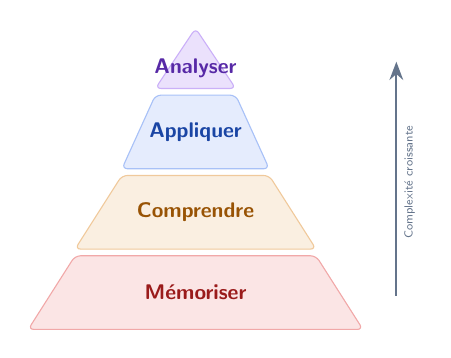
\begin{tikzpicture}[scale=0.85, every node/.style={transform shape}]
    \filldraw[fill=danger!12, draw=danger!40, rounded corners=2pt]
      (0,0) -- (5,0) -- (4.3,1.1) -- (0.7,1.1) -- cycle;
    \filldraw[fill=warning!12, draw=warning!40, rounded corners=2pt]
      (0.7,1.2) -- (4.3,1.2) -- (3.6,2.3) -- (1.4,2.3) -- cycle;
    \filldraw[fill=primary!12, draw=primary!40, rounded corners=2pt]
      (1.4,2.4) -- (3.6,2.4) -- (3.1,3.5) -- (1.9,3.5) -- cycle;
    \filldraw[fill=secondary!15, draw=secondary!40, rounded corners=2pt]
      (1.9,3.6) -- (3.1,3.6) -- (2.5,4.5) -- cycle;

    \node[font=\small\sffamily\bfseries, text=danger!70!black] at (2.5,0.55) {M\'emoriser};
    \node[font=\small\sffamily\bfseries, text=warning!70!black] at (2.5,1.75) {Comprendre};
    \node[font=\small\sffamily\bfseries, text=primary!70!black] at (2.5,2.95) {Appliquer};
    \node[font=\small\sffamily\bfseries, text=secondary!70!black] at (2.5,3.9) {Analyser};

    \draw[-{Stealth}, thick, gentlegray] (5.5,0.5) -- (5.5,4);
    \node[font=\tiny\sffamily, text=gentlegray, rotate=90, anchor=south]
      at (5.9,2.2) {Complexit\'e croissante};
  \end{tikzpicture}
\end{column}
\begin{column}{0.48\textwidth}
  \begin{block}{Application dans le Quiz}
    Chaque concept extrait est tagg\'e avec un \textbf{niveau de Bloom}~:
    \begin{itemize}\small
      \item \textbf{M\'emoriser} --- rappeler un fait\\
        {\scriptsize Ex~: ``Quelle est la formule de l'eau~?''}
      \item \textbf{Comprendre} --- expliquer un concept\\
        {\scriptsize Ex~: ``Expliquez le r\^ole des enzymes.''}
      \item \textbf{Appliquer} --- utiliser dans un nouveau contexte\\
        {\scriptsize Ex~: ``Calculez le pH d'une solution.''}
      \item \textbf{Analyser} --- d\'ecomposer les relations\\
        {\scriptsize Ex~: ``Comparez la mitose et la m\'eiose.''}
    \end{itemize}
  \end{block}

  \begin{alertblock}{Adaptation}
    \small Un concept \textbf{ma\^itris\'e} est pouss\'e vers un niveau sup\'erieur (\emph{stretch}).
    Un concept \textbf{en difficult\'e} est renforc\'e au m\^eme niveau.
  \end{alertblock}
\end{column}
\end{columns}
\end{frame}

% ══════════════════════════════════════════════════════════════════════
\subsection{Agent Flashcard}
% ══════════════════════════════════════════════════════════════════════

\begin{frame}{Agent Flashcard --- Cartes M\'emoire Intelligentes}
\begin{columns}[T]
\begin{column}{0.48\textwidth}
  Cet agent g\'en\`ere des \textbf{cartes m\'emoire} \`a partir des documents, avec planification de r\'evision par \textbf{r\'ep\'etition espac\'ee}.

  \bigskip
  \begin{block}{Pipeline en 8 \'etapes}
    \begin{enumerate}
      \item \textbf{Mining de concepts (spaCy)} --- extraction automatique des termes cl\'es via NER, chunks nominaux, et patterns regex (``X est Y'').

      {\scriptsize \textbf{spaCy~:} biblioth\`eque NLP. \textbf{NER~:} Named Entity Recognition --- identification automatique d'entit\'es (noms, lieux, concepts) dans un texte.}

      \item \textbf{Filtrer le bruit} --- \'eliminer auteurs, num\'eros de page, URLs, copyright par regex.

      \item \textbf{Prioriser} --- les concepts en \emph{difficult\'e} d'abord, puis les plus fr\'equents.

      \item \textbf{Cartes Q\&R} --- le LLM g\'en\`ere des paires question-r\'eponse en JSON structur\'e.
    \end{enumerate}
  \end{block}
\end{column}
\begin{column}{0.48\textwidth}
  \begin{block}{Suite du pipeline}
    \begin{enumerate}
      \setcounter{enumi}{4}
      \item \textbf{Cartes Cloze} --- transformation par regex~: le terme cl\'e est remplac\'e par un trou.

      {\scriptsize Ex~: ``\underline{\hspace{1cm}} est le processus par lequel les plantes convertissent la lumi\`ere\ldots''}

      \item \textbf{D\'edoublonner} --- \'eliminer les cartes quasi-identiques par chevauchement de tokens.

      \item \textbf{Planification SM-2} --- attacher les m\'etadonn\'ees de r\'ep\'etition espac\'ee.

      \item \textbf{Exporter} --- JSON $\rightarrow$ MinIO $\rightarrow$ rendu dans le frontend.
    \end{enumerate}
  \end{block}

  \begin{exampleblock}{Lien avec le RAG}
    \small Utilise le mode \textbf{coverage\_broad} pour diversifier.
    Le mining par spaCy est \textbf{100$\times$ plus rapide} qu'un appel LLM.
  \end{exampleblock}
\end{column}
\end{columns}
\end{frame}

% ──────────────────────────────────────────────────────────────────────
\begin{frame}{Concept Cl\'e~: R\'ep\'etition Espac\'ee (SM-2)}
\begin{columns}[T]
\begin{column}{0.48\textwidth}
  \textbf{SM-2} (SuperMemo 2) est l'algorithme derri\`ere les syst\`emes de cartes m\'emoire comme \textbf{Anki}.

  \bigskip
  \begin{block}{Principe}
    Plut\^ot que de r\'eviser toutes les cartes chaque jour~:
    \begin{itemize}
      \item Une carte \textbf{bien retenue} est r\'evis\'ee \textbf{plus tard} (intervalles croissants~: 1j $\rightarrow$ 3j $\rightarrow$ 7j $\rightarrow$ 15j\ldots)
      \item Une carte \textbf{oubli\'ee} est r\'evis\'ee \textbf{imm\'ediatement}
    \end{itemize}

    \smallskip
    {\small R\'esultat~: un \textbf{minimum d'effort} pour une \textbf{r\'etention maximale}.}
  \end{block}

  \bigskip
  \begin{block}{Param\`etres attach\'es \`a chaque carte}
    \begin{itemize}
      \item \textbf{Facteur de facilit\'e}~: 2.5 (initial)
      \item \textbf{Intervalle}~: 1 jour (initial)
      \item \textbf{Horodatage \texttt{due\_at}}~: quand r\'eviser
    \end{itemize}
  \end{block}
\end{column}
\begin{column}{0.48\textwidth}
  \centering
  \textbf{\'Evolution des intervalles de r\'evision}

  \bigskip
  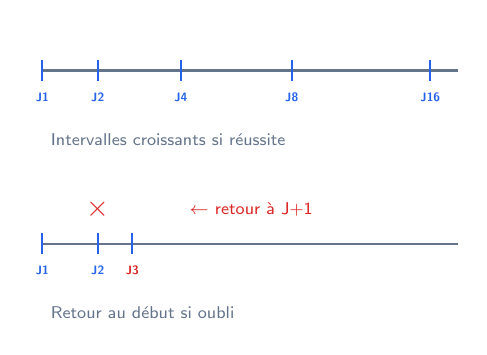
\begin{tikzpicture}[scale=0.88, every node/.style={transform shape}]
    % Timeline
    \draw[thick, gentlegray] (0,0) -- (6,0);

    % Ticks
    \foreach \x/\d in {0/J1, 0.8/J2, 2/J4, 3.6/J8, 5.6/J16} {
      \draw[thick, primary] (\x,-0.15) -- (\x,0.15);
      \node[font=\tiny\sffamily\bfseries, text=primary, below] at (\x,-0.2) {\d};
      \node[font=\large, text=accent] at (\x,0.5) {$\checkmark$};
    }

    \node[font=\scriptsize\sffamily, text=gentlegray, anchor=west] at (0,-1)
      {Intervalles croissants si r\'eussite};

    % Forgot scenario
    \draw[thick, gentlegray] (0,-2.5) -- (6,-2.5);
    \draw[thick, primary] (0,-2.65) -- (0,-2.35);
    \node[font=\tiny\sffamily\bfseries, text=primary, below] at (0,-2.7) {J1};
    \node[font=\large, text=accent] at (0,-2) {$\checkmark$};

    \draw[thick, primary] (0.8,-2.65) -- (0.8,-2.35);
    \node[font=\tiny\sffamily\bfseries, text=primary, below] at (0.8,-2.7) {J2};
    \node[font=\large, text=danger] at (0.8,-2) {$\times$};

    \draw[thick, primary] (1.3,-2.65) -- (1.3,-2.35);
    \node[font=\tiny\sffamily\bfseries, text=danger, below] at (1.3,-2.7) {J3};
    \node[font=\large, text=accent] at (1.3,-2) {$\checkmark$};

    \node[font=\scriptsize\sffamily, text=danger, anchor=west] at (2,-2)
      {$\leftarrow$ retour \`a J+1};

    \node[font=\scriptsize\sffamily, text=gentlegray, anchor=west] at (0,-3.5)
      {Retour au d\'ebut si oubli};
  \end{tikzpicture}

  \bigskip
  \begin{alertblock}{Int\'er\^et pour TeacherLM}
    \small Les cartes sont g\'en\'er\'ees avec les m\'etadonn\'ees SM-2 \textbf{d\`es la cr\'eation}. Le frontend peut ensuite planifier les r\'evisions automatiquement.
  \end{alertblock}
\end{column}
\end{columns}
\end{frame}

% ══════════════════════════════════════════════════════════════════════
\section{Suivi de l'Apprenant}
% ══════════════════════════════════════════════════════════════════════

\begin{frame}{Suivi de Ma\^itrise par Concept}
\begin{columns}[T]
\begin{column}{0.48\textwidth}
  Chaque conversation maintient un \textbf{mod\`ele de ma\^itrise} qui suit la progression de l'\'etudiant concept par concept.

  \bigskip
  \begin{block}{Mise \`a jour apr\`es chaque interaction}
    \textbf{L'\'etudiant d\'emontre la compr\'ehension~:}
    $$m' = m + 0{,}2 \times (1 - m)$$
    {\small Rendements d\'ecroissants --- chaque d\'emonstration compte moins \`a mesure qu'on s'approche de 1.}

    \bigskip
    \textbf{L'\'etudiant montre de la confusion~:}
    $$m' = m \times 0{,}7$$
    {\small D\'ecroissance multiplicative --- la ma\^itrise diminue rapidement.}
  \end{block}

  \begin{block}{Seuils de classification}
    \begin{itemize}
      \item $m \geq 0{,}7$ $\rightarrow$ concept \og{} \textbf{ma\^itris\'e} \fg{}
      \item $m \leq 0{,}3$ $\rightarrow$ concept \og{} \textbf{en difficult\'e} \fg{}
    \end{itemize}
  \end{block}
\end{column}
\begin{column}{0.48\textwidth}
  \begin{block}{Impact sur chaque agent}
    \renewcommand{\arraystretch}{1.4}
    \begin{tabular}{>{\bfseries\color{secondary}\small}l p{5cm}}
      \toprule
      Agent & Utilisation de l'\'etat \\
      \midrule
      Enseignant & Choisit le \textbf{mode de r\'eponse}~: expliquer si bloqu\'e, guider si confus, affirmer si ma\^itris\'e \\
      Quiz & \textbf{60\%} des questions ciblent les concepts en difficult\'e ; 10\% de d\'efi pour les concepts ma\^itris\'es \\
      Flashcard & Les concepts en difficult\'e sont \textbf{prioritaires} dans le deck g\'en\'er\'e \\
      \bottomrule
    \end{tabular}
  \end{block}

  \bigskip
  \begin{exampleblock}{Boucle de r\'etroaction}
    \small Apr\`es chaque interaction, le LLM (3B) extrait les concepts d\'emontr\'es / en difficult\'e. L'\'etat est mis \`a jour et influence la \textbf{prochaine} interaction.
  \end{exampleblock}
\end{column}
\end{columns}
\end{frame}

% ══════════════════════════════════════════════════════════════════════
\section{Scoring de Confiance}
% ══════════════════════════════════════════════════════════════════════

\begin{frame}{Ancrage et Scoring de Confiance}
\begin{columns}[T]
\begin{column}{0.48\textwidth}
  Apr\`es chaque r\'eponse g\'en\'er\'ee, le syst\`eme mesure sa \textbf{qualit\'e}~:

  \bigskip
  \begin{block}{Score d'Ancrage\\ {\small(\emph{Groundedness})}}
    Pour chaque phrase de la r\'eponse, on calcule le \textbf{chevauchement de tokens} avec les chunks sources~:

    $$\text{ancrage} = \frac{1}{|S|} \sum_{s \in S} \frac{|\text{tokens}(s) \cap \text{vocab}|}{|\text{tokens}(s)|}$$

    \begin{itemize}\small
      \item Proche de 1{,}0 $\rightarrow$ bien ancr\'e dans les documents
      \item Proche de 0{,}0 $\rightarrow$ hallucination potentielle
    \end{itemize}
  \end{block}

  \begin{block}{Score de Couverture}
    Quelle fraction des mots-cl\'es de la question apparaissent dans les chunks r\'ecup\'er\'es~?

    \smallskip
    {\small V\'erifie que la recherche a bien \textbf{captur\'e le sujet} de la question.}
  \end{block}
\end{column}
\begin{column}{0.48\textwidth}
  \begin{block}{Garde Hors-Sujet}
    Si le meilleur score du cross-encoder pour une question est \textbf{tr\`es bas} (< seuil)~:

    \smallskip
    $\rightarrow$ L'agent \textbf{refuse poliment} de r\'epondre.

    \smallskip
    \emph{``Ce sujet ne semble pas couvert par vos documents t\'el\'evers\'es.''}

    \bigskip
    {\small \textbf{Pourquoi~?} Mieux vaut admettre ne pas savoir que de g\'en\'erer une r\'eponse non ancr\'ee. C'est la \textbf{garantie fondamentale} du syst\`eme.}
  \end{block}

  \bigskip
  \centering
  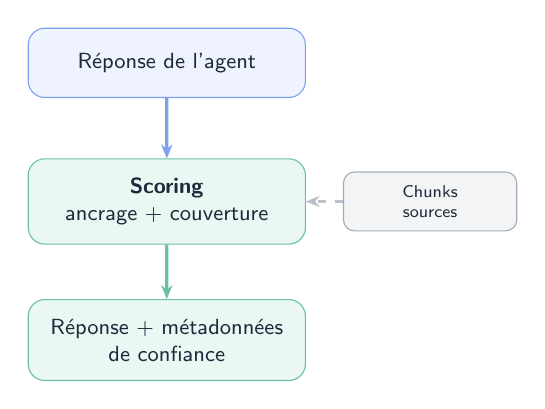
\begin{tikzpicture}[scale=0.88, every node/.style={transform shape}]
    \node[wbox=primary, minimum width=4cm] (resp) at (0,2)
      {R\'eponse de l'agent};

    \node[wbox=accent, minimum width=4cm] (score) at (0,0)
      {\textbf{Scoring}\\ancrage + couverture};

    \node[box=gentlegray, minimum width=2.5cm] (ch) at (3.8,0)
      {Chunks\\sources};

    \node[wbox=accent, minimum width=4cm] (out) at (0,-2)
      {R\'eponse + m\'etadonn\'ees\\de confiance};

    \draw[arr, line width=1.2pt] (resp) -- (score);
    \draw[darr] (ch) -- (score);
    \draw[arr=accent, line width=1.2pt] (score) -- (out);
  \end{tikzpicture}
\end{column}
\end{columns}
\end{frame}

% ══════════════════════════════════════════════════════════════════════
\section{\'Etat d'Avancement}
% ══════════════════════════════════════════════════════════════════════

\begin{frame}{\'Etat d'Avancement Actuel}
\begin{columns}[T]
\begin{column}{0.48\textwidth}
  \begin{block}{R\'ealis\'e \checkmark}
    \begin{itemize}
      \item[\color{accent}\checkmark] Pipeline RAG complet (ingestion + r\'ecup\'eration hybride + reranking)
      \item[\color{accent}\checkmark] 3 agents fonctionnels (enseignant, quiz, flashcard)
      \item[\color{accent}\checkmark] Suivi de ma\^itrise apprenant
      \item[\color{accent}\checkmark] Scoring de confiance et garde hors-sujet
      \item[\color{accent}\checkmark] Architecture plugin (registre JSON)
      \item[\color{accent}\checkmark] Frontend Next.js (chat, quiz, flashcard renderers)
      \item[\color{accent}\checkmark] Docker Compose (10 services)
      \item[\color{accent}\checkmark] LLM enti\`erement local (Ollama)
    \end{itemize}
  \end{block}
\end{column}
\begin{column}{0.48\textwidth}
  \begin{block}{En cours / Pr\'evu}
    \begin{itemize}
      \item[$\circ$] Agent Mindmap (diagrammes de concepts)
      \item[$\circ$] Agent Podcast (explications audio)
      \item[$\circ$] Agent Report (r\'esum\'es structur\'es)
      \item[$\circ$] Am\'elioration de la qualit\'e des quiz
      \item[$\circ$] Sessions de r\'evision SM-2 dans le frontend
      \item[$\circ$] Tests automatis\'es end-to-end
    \end{itemize}
  \end{block}

  \bigskip
  \begin{exampleblock}{Technologies cl\'es}
    \small
    \textbf{Backend~:} Python, FastAPI, Ollama, Qdrant, fastembed\\
    \textbf{Frontend~:} Next.js 14, React, TailwindCSS\\
    \textbf{Infra~:} Docker Compose, PostgreSQL, Redis, MinIO
  \end{exampleblock}
\end{column}
\end{columns}
\end{frame}

% ══════════════════════════════════════════════════════════════════════
\section{R\'esum\'e}
% ══════════════════════════════════════════════════════════════════════

\begin{frame}{R\'esum\'e}
\centering
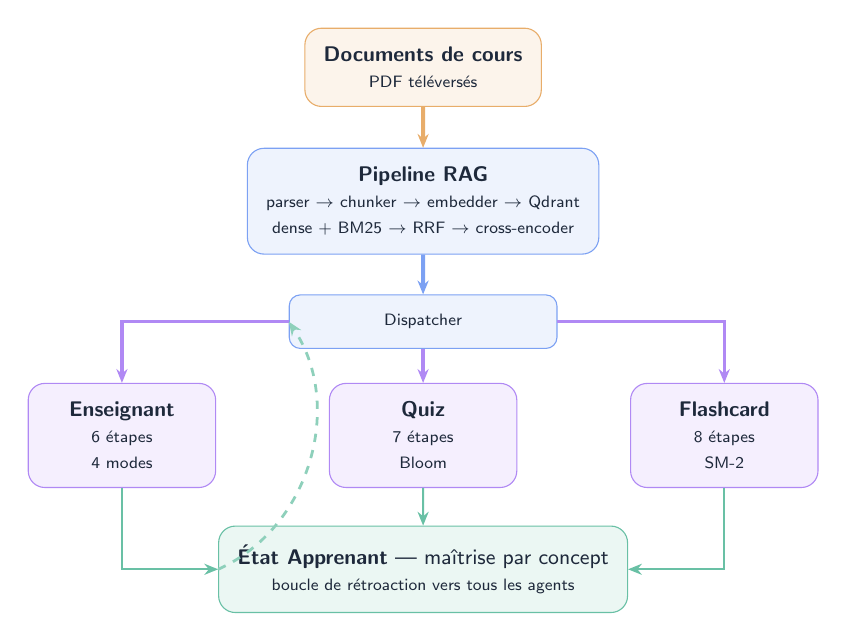
\begin{tikzpicture}[scale=0.85, every node/.style={transform shape}]
  % Flow
  \node[wbox=warning, minimum width=3.5cm] (docs) at (0,4)
    {\textbf{Documents de cours}\\{\scriptsize PDF t\'el\'evers\'es}};

  \node[wbox=primary, minimum width=5cm] (rag) at (0,2)
    {\textbf{Pipeline RAG}\\{\scriptsize parser $\rightarrow$ chunker $\rightarrow$ embedder $\rightarrow$ Qdrant}\\
     {\scriptsize dense + BM25 $\rightarrow$ RRF $\rightarrow$ cross-encoder}};

  \node[box=primary, minimum width=4cm, minimum height=0.8cm] (disp) at (0,0.2)
    {Dispatcher};

  \node[wbox=secondary, minimum width=2.8cm] (t) at (-4.5,-1.5)
    {\textbf{Enseignant}\\{\scriptsize 6 \'etapes}\\{\scriptsize 4 modes}};
  \node[wbox=secondary, minimum width=2.8cm] (q) at (0,-1.5)
    {\textbf{Quiz}\\{\scriptsize 7 \'etapes}\\{\scriptsize Bloom}};
  \node[wbox=secondary, minimum width=2.8cm] (f) at (4.5,-1.5)
    {\textbf{Flashcard}\\{\scriptsize 8 \'etapes}\\{\scriptsize SM-2}};

  \node[wbox=accent, minimum width=5cm] (ls) at (0,-3.5)
    {\textbf{\'Etat Apprenant} --- ma\^itrise par concept\\
     {\scriptsize boucle de r\'etroaction vers tous les agents}};

  \draw[arr=warning, line width=1.5pt] (docs) -- (rag);
  \draw[arr, line width=1.5pt] (rag) -- (disp);
  \draw[arr=secondary, line width=1.2pt] (disp) -| (t);
  \draw[arr=secondary, line width=1.2pt] (disp) -- (q);
  \draw[arr=secondary, line width=1.2pt] (disp) -| (f);
  \draw[arr=accent] (t) |- (ls);
  \draw[arr=accent] (q) -- (ls);
  \draw[arr=accent] (f) |- (ls);
  \draw[darr=accent, line width=1pt, bend right=50] (ls.west) to (disp.west);
\end{tikzpicture}
\end{frame}

% ─── MERCI ────────────────────────────────────────────────────────────
{
\setbeamertemplate{footline}{}
\begin{frame}
\centering
\vfill
{\Huge\bfseries\color{primary} Merci}

\bigskip
{\large\color{gentlegray} Questions~?}

\vfill
{\small\color{gentlegray}
TeacherLM --- Pr\'esentation d'\'etat d'avancement
}
\vfill
\end{frame}
}

\end{document}
